\chapter{Technische Herausforderungen der Blockchain/smarter Verträge}
\section{Herausforderungen auf Basis von Wallets}
\subsection{Diebstahl von Wallets}
Wie auch bei zentralen Diensten muss ein Nutzer sein Passwort schützen. Bei Bitcoin-Wallets besteht das Problem, dass es ausreicht an den privaten Schlüssel zu kommen, um als Angreifer Macht über das gesamte Konto zu erlangen. Theoretisch ist die Wahrscheinlichkeit einen privaten Schlüssel zu erraten sehr gering, praktisch hängt es von der gewählten Passphrase ab, auf die der ECDSA-Algorithmus angewandt wird. Korantin Auguste stellt in einem Blogbeitrag dar, wie durch die Verwendung kleiner Zahlen oder von Beispielsätzen (sogenannten Brainwallets) bereits erfolgreich Attacken auf Wallets verübt worden sind. \\
Außerdem ist es möglich durch den Einsatz von Malware, Phishing Tools, Social Engineering, etc. direkt an den Besitz des privaten Schlüssels zu gelangen.

Einen besseren Schutz bietet Ethereum. Hier muss bei der Erstellung eines Wallets zusätzlich noch ein Passwort angegeben werden. Mit diesem wird der private Schlüssel verschlüsselt. Dadurch muss ein Angreifer, wenn er in den Besitz des verschlüsselten Schlüssels gelangt zusätzlich noch das Passwort erraten.

\subsection{Verlust von Wallets}
Verliert ein Nutzer seinen privaten Schlüssel, so verliert er auch jede Zugriffsmöglichkeit auf das Wallet. Da es keine zentrale Instanz gibt, die den Schlüssel wiederherstellen kann, ist das Wallet unwiderruflich Verloren. Werden Coins an ein solches Wallet überwiesen, sind auch diese verloren.
\section{Skalierbarkeit}
\section{Fehlende Belohnungen für die Nutzung von Full Nodes}
Full Nodes sind bei der Blockchain-Technologie ein wichtiger Baustein um Qualität und Sicherheit des Netzwerks sicherzustellen. Sie Überprüfen unter anderem die Gültigkeit einer propagierten Blockchain, versorgen andere Nodes mit Informationen über die Blöcke und stehen für Light Nodes für den Merkle-Proof zur Verfügung.

Das Betreiben eines Full Nodes sorgt daher bei dem Nutzer für eine höhere Sicherheit und Anonymität als die Verwendung eines Light Nodes. Für die meisten Nutzer ist es jedoch vollkommen ausreichend einen Light Node zu betreiben, weshalb bei Bitcoin die Anzahl an Full Nodes stark abnehmend ist. Ohne zusätzliche Belohnungen, die Strom und Hardwarekosten kompensieren lohnt sich das Betreiben eines Full Nodes für den durchschnittlichen Nutzer nicht.
\section{Kompatibilität von Blockchains}
\section{Anbindung von Schnittstellen}
\section{Light Nodes}
durch \ac{SPV} kann nur festgestellt werden, ob eine Transaktion tatsächlich durchgeführt worden ist. Um sicherzustellen, dass diese Transaktion nicht doppelt ausgeführt wurde (double spending), muss ein \ac{SPV} bei mehreren Nodes nachfragen, um die Wahrscheinlichkeit zu erhöhen, dass einer dieser Nodes ein ehrlicher ist und nicht der eines Angreifers. \\
Dadurch ist ein \ac{SPV} angreifbar durch partitoning attacks oder sybil attacks. \cite{Antonopoulos.2015}[S.149]
\section{Sicherheit}
\subsection{Sybil-Attacke}
\subsection{Selfish-Mining}
\subsection{51\% Attacke}
Die 51\% Attacke umschreibt einen Angriff, in dem ein Angreifer 51\% der Rechenleistung des Netzwerks aufbringt. Dadurch hat der Angreifer eine höhere Wahrscheinlichkeit, neue Blöcke zu bilden als der Rest des Netzwerks. Durch nicht-Veröffentlichung der gefundenen Blöcke kann er eine parallele Blockchain bilden, die länger als die von den ehrlichen Minern erarbeitete ist. Sobald er diese veröffentlicht, wird nach der "longest chain rule", welche besagt, dass immer der längsten Kette gefolgt wird, sofort von allen Minern von der bekannten Chain auf die des Angreifers gewechselt. \cite{Nakamoto.31.10.2008}[S.3] Doch welche Möglichkeiten ergeben sich nun für den Angreifer?
\begin{enumerate}
	\item Der Angreifer kann alle oder eine Teilmenge aller ab der Teilung der Kette getätigten Transaktionen rückgängig machen
	\item Der Angreifer kann ein \glqq double spending\grqq{} durchführen, indem er in der \glqq ehrlichen\grqq{} Kette eine Transaktion ausführt bis sie vom Empfänger als gültig akzeptiert wird und diese dann in seiner \glqq neuen\grqq{} Kette rückgängig macht. Dadurch geht die \ac{UTXO} auf sein Konto zurück und er kann die Geldeinheiten wiederholt ausgeben.
\end{enumerate}

Nach dem Bitcoin-Design von Satoshi Nakamoto soll durch das Mining sichergestellt werden, dass viele Miner, die jeweils einen kleinen Anteil an der gesamten Rechenleistung haben, es für einen Angreifer zu kostenintensiv ist eine solche Attacke auszuüben. Zusätzlich wird von ihm angenommen, dass die Belohnungen für ehrliches Mining höher sind, als die die durch Angriffe erzielt werden können. Insbesondere da bei einem erfolgreichen Angriff der Wert der Währung massiv sinken würde.
 Durch das Einführen von sogenannten ASIC-Minern \footnote{http://asicminer-shop.de/Bitmain-Antminer-S7-486-TH-s-Gebrauchtgeraet} mit Hashraten von mehreren Tera-Hashes pro Sekunde, wurde das normale Mining auf klassischen Rechnern nicht mehr profitabel. \todo{Begründung oder Quelle}
Für diejenigen, die trotzdem noch Minen oder in einen ASIC-Miner investiert haben besteht zusätzlich noch das Problem eines sehr unregelmäßigen Kapitalrückflusses. Mit ca 1.200.000 Tera Hashes pro Sekunde \footnote{https://blockchain.info/de/charts/hash-rate} ist es relativ unwahrscheinlich selbst einen Block zu lösen. Daher haben sich viele Miner in Mining-Pools zusammengeschlossen (siehe Mining Pools) \todo{Referenz}

\begin{figure}[ht]
	\centering
	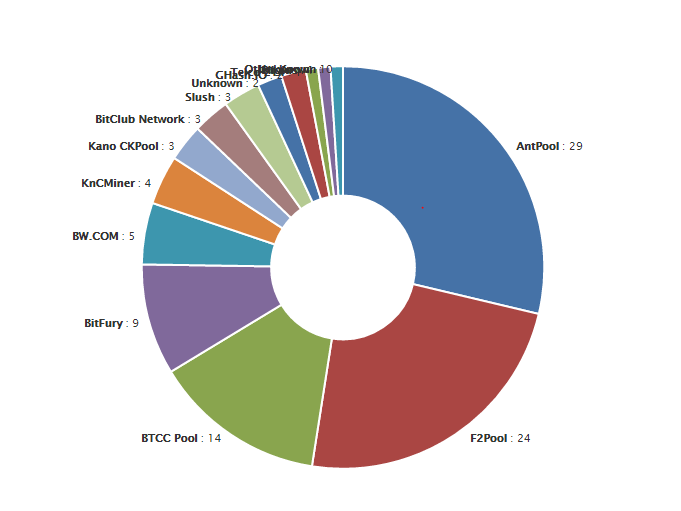
\includegraphics[scale=0.75]{grafiken/mining_pool_verteilung.png}
	\caption{Verteilung der Bitcoin Mining pools }
	\label{mining_pool_verteilung}
\end{figure}
\todo{Quelle}
Abbildung \ref{mining_pool_verteilung} zeigt, das bereits 2 der größten Mining Pools mehr als 50\% der Mining Power besitzen. Ein möglicher Angriff wäre beispielsweise die Server der Pool Manager zu hacken. Doch auch ein Angriff mit eigener Hardware wäre für einige Organisationen möglich. James D'Angelo beschreibt in einer 2-teiligen Youtube Serie mögliche Organisationen, die für bereits ab 20 Millionen Euro kosten eine mögliche Gefahr für das Bitcoin Netzwerk darstellen können. Dazu zählen hauptsächlich die Hersteller von Mining Computern. \cite{Angelo.2014} \cite{Angelo.2014b}\\

Ein Angriff aus finanziellen Gründen ist jedoch sehr unwahrscheinlich. Die einzige Motivation wäre das Durchführen von \glqq double spending\grqq{} Angriffen. Diese wären selbst für einen Chip-Hersteller vergleichsweise teuer und auch wenn ein solcher Angriff auf der Chain nicht ersichtlich ist, würden die geschädigten Parteien wohl sehr schnell den Betrug propagieren. Ein vorstellbares Szenario wäre jedoch der Versuch, die Währung als ganzes zu zerstören. Insbesondere Staaten wie Russland und China, die eine sehr restriktive Geldpolitik haben und befürchten, dass die Bürger ihre Einlagen in Crypto-Währungen sichern, hätten hierzu eine deutliche Motivation. Sie könnten für eine längere Zeit mit 51\% der Rechenpower eine Chain mit keinen oder nur sehr wenigen Transaktionen mitführen. Da zum Zeitpunkt der Veröffentlichung in die neue Chain gewechselt würde, würden wie beschrieben alle bis zum Zeitpunkt des Forks getätigten Transaktionen zurück gerollt werden, was Crypto-Währungen als Zahlungssystem wahrscheinlich zumindest für einige Jahre obsolet machen würde.
\subsection{Notizen}
\begin{itemize}
	\item Wucherungen des Hauptbuchs. Jedes Wallet muss eine Kopie des Hauptbuchs herunterladen. Diese wächst mit Bekanntheit der Anwendung. Insbesondere problematisch für mobile Anwendungen
	\item Tendenz zur Monopolisierung des Netzwerks in einem einzigen Mining Pool
	\item Tendenz zur Zentralisierung der Geldmenge
	\item Wie viel des Netzwerkes benötige ich um die Blockchain zu „Kapern“? Was sind die Auswirkungen?
	\item Code als Single-Point-of-Failure. Wie kann – insbesondere bei programmierbaren Coins Sicherheit gewährleistet werden?
	\item Bei Smart contracts kann jeder die Vertragsbedingungen (bzw. den gecodeten Vetrag) einsehen. Dies kann z.B. zu einem Interessenkonflikt mit anderen Vertragspartnern führen. Welche Möglichkeiten, dass zu unterbinden bestehen?
	\item Schutz durch Proof-of-work. Annahme: Bitcoin-miner haben ausschlie{\ss}lich finanzielle Interessen. Ihr Verdienst ist die Belohnung durch das Lösen von Blöcken. d.h. Gewinn = Belohnung – Mining-kosten
	Will jemand (Eve) das Netzwerk übernehmen, besticht er die Mining-Pools. Diese haben dadurch keine extra-kosten, Eve hat folgende Gewinn-Funktion: Gewinn = Belohnung durch übernehmen des Netzwerks – Kosten für Bestechung der Mining-Pools. 
	diese Kosten sind bei der Annahme rein finanzieller Interessen >= 0
	\item Sybil attack
\end{itemize}
\section{Resümee}